\subsection{Syntax-number units connections}

\begin{figure*}[t]
    \centering
    \begin{subfigure}{0.49\textwidth}
            \centering
            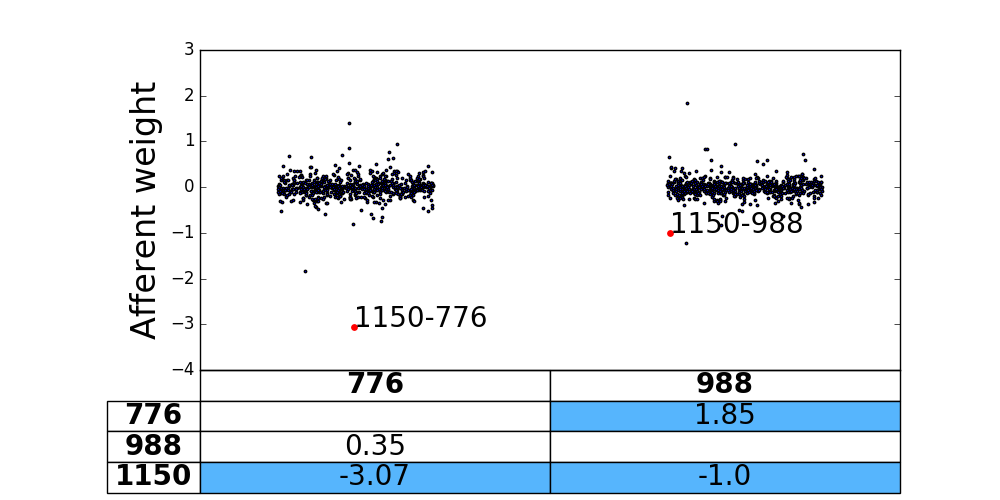
\includegraphics[width=\textwidth]{Figures/gate_Input_afferent_interactions.png}
            \caption{Input gate}
            \label{fig:interaction-input}
    \end{subfigure}
    \begin{subfigure}{0.49\textwidth}
           \centering
          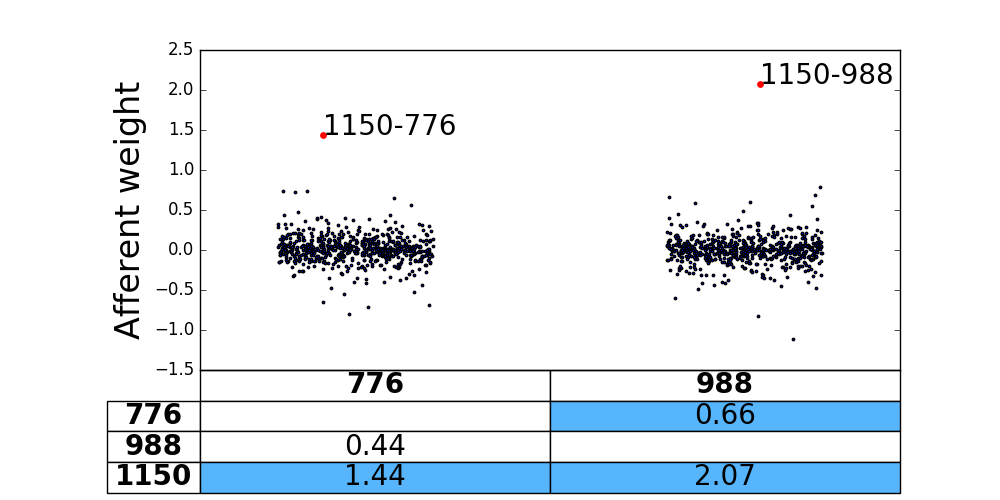
\includegraphics[width=\textwidth]{Figures/gate_Forget_afferent_interactions.png}
          \caption{Forget gate}
          \label{fig:interaction-forget}
    \end{subfigure}
\caption{Connections to syntax unit \unit{2}{500} and LR-number units \unit{2}{126} and \unit{2}{338}. \marco{ put more extended caption (possibly moving stuff from text).}}\yair{remove third column and distribution? Figure could then be compressed to linewidth}
\label{fig:interaction}
\end{figure*}

We finally look at the connections that were learned by the LSTM
between syntax unit \unit{2}{500}, which appears to be more closely involved in
tracking subject-verb agreement, and the number units, as well as at
the connections between the latter. For each unit pair, there are 4
connection types, one for each component of the target cell (to the 3
gates and to the memory cell). We focus on input and forget gates, as they control the flow and storage of number information.

% The previous sections described two crucial factors required to solve the NA-task by the network - units that encode and carry the subject number across long-range dependencies, and a unit that encodes the main subject-verb dependency. We now look into the interactions among these units by analyzing the weights in the network. We note that for each pair of units there are four types of connections corresponding to the four types of gates in the units. Each type of weight can thus contribute to a different type of interaction, depending on the function of the gate. 

Figures \ref{fig:interaction-input} and \ref{fig:interaction-forget} show the distributions of all afferent recurrent weights to the number units input and forget gates. Weights from the syntax units are marked in red and are labeled. Table values represent weight sizes among the units (projecting units appear to the left of the table), and blue background represents that the corresponding weight is an outlier ($|z-score|>3$). Results show that the weight values from the syntax unit to the forget gate of both \unit{2}{126} and \unit{2}{338} are exceptionally high compared to all other afferent connections in the network ($z-score=3.5, 5.1$, respectively), and exceptionally negative to their input gates ($z-score=-10.0, -3.1$). \marco{It looks like previous description pertains to an older plot.} \yair{why?}

Since cell activity of syntax unit X is positive across the entire
subject-verb dependency (e.g., Figure
\ref{fig:syntax-unit-double-subjrel}), the connectivity from the
syntax unit drives the number unit forget gates towards 1
($W^f_{776, 1150}h_{1150}>0$) and their input gates towards 0
($W^i_{776, 1150}h_{1150}<0$). Looking at the right-hand-side of
Eq.~(\ref{eq:update-rule}), this means that the first term becomes
  dominant and the second vanishes, suggesting that, across the entire
  dependency the syntax unit conveys a \textit{`remember flag'}
  to the number units, and, similarly, when the activity of the syntax
  unit becomes negative, it conveys an \textit{`update
    flag'} at the end of the dependency.

Last, we note that the weight values between the two number units are significantly high compared to all other afferent connections. Since their activity is negative across the dependency (Figure \ref{fig:singular-unit} and \ref{fig:plural-unit}), this means that they are \textit{mutually inhibiting}, thus warranting an unequivocal signal about the grammatical number of the subject to the output layer.

